\section{Warm up: Support Vector Machines}
\label{sec:svm}

In class you have seen support vector machines (SVMs).  Here we will find the optimal classifier of a simple dataset by hand.  Assume that we are given the following dataset:
\begin{align*}
\mathcal{D}_+ &= \begin{bmatrix}
  3 & \phantom{-}1\\
  3 & -1\\
  6 & \phantom{-}1\\
  6 & -1
\end{bmatrix}
&& \mathcal{D}_-= \begin{bmatrix}
  \phantom{-}1 & \phantom{-}0\\
  \phantom{-}0 & \phantom{-}1\\
  \phantom{-}0 & -1\\
  -1 & \phantom{-}0
\end{bmatrix}
\end{align*}
where $\mathcal{D}_+$ are positive examples and $\mathcal{D}_-$ are negative examples.
\begin{enumerate}
\item ~[9 points] Find the optimal hyperplane and the corresponding
  maximum margin. Which training points are the support vectors?

\begin{itemize}
\item The solution is the hyperplane about $y=2$, which can be seen in Figure~\ref{fig:1a}, where the support vectors are from the positive as $(3,1)$ and $(3,-1)$ as they both have the same distance to the hyperplane, and for the negatives $(1, 0)$. It is the maximized margin between both points (the midpoint between them) as the distance of each closest point to the hyperplane is $1$.
\end{itemize}

\item ~[2 points] You are given a new point $x = [1.8,1]$ with true
  label -1. Does your SVM correctly classify this point?

\begin{itemize}
\item Yes, please refer to Figure~\ref{fig:1b}
\end{itemize}  



\item ~[4 points] Now let's compare this classifier to the vanilla
  Perceptron algorithm. Assume that we have the point $x = [1.9999,1]$
  with label -1. If we allow the Perceptron algorithm to run until it
  achieves 0\% error on the training set will it be guarenteed to
  classify this point correctly? Why or why not justify your answer.

\begin{itemize}
\item I talked with Dr. Srikumar and he said that this question is to be taken as you {\em learn} on the original 8 points, and the $(1.999,1)$ point is to be the ``test'' point. 

The vanilla Perceptron algorithm will not necessairly classify the last point correctly. The normal Perceptron algorithm does not care about the resulting weight vector, only that the training set is classified correctly. Figure~\ref{fig:1c} shows and example of how the training set could be classified correctly, but it wouldn't classify the test point $(1.999,1)$ correctly.
\end{itemize}  


\end{enumerate}

\begin{figure}[!h]
\centering
\begin{minipage}{.5\textwidth}
  \centering
  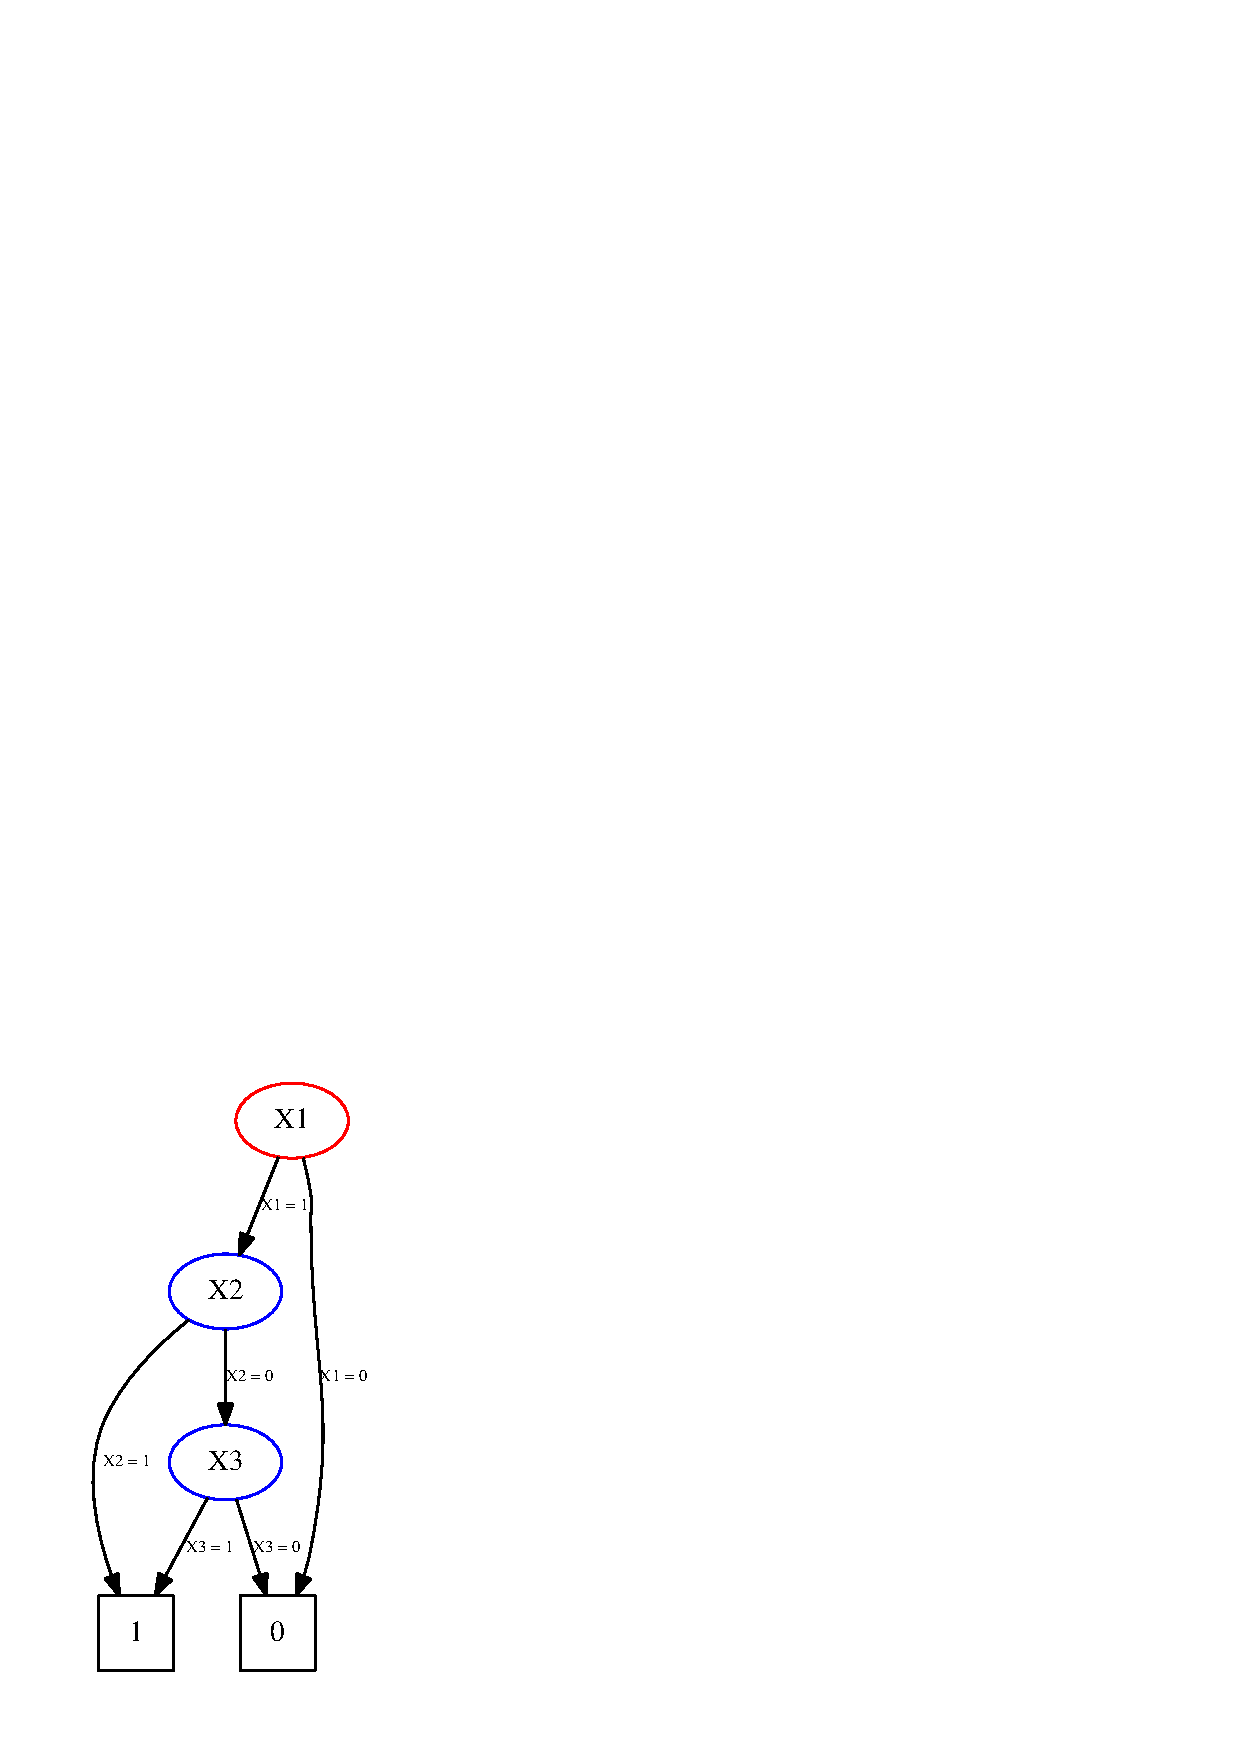
\includegraphics[width=\linewidth]{progs/1a.pdf}
  \captionof{figure}{Solution to Problem 1}
  \label{fig:1a}
\end{minipage}%
\begin{minipage}{.5\textwidth}
  \centering
  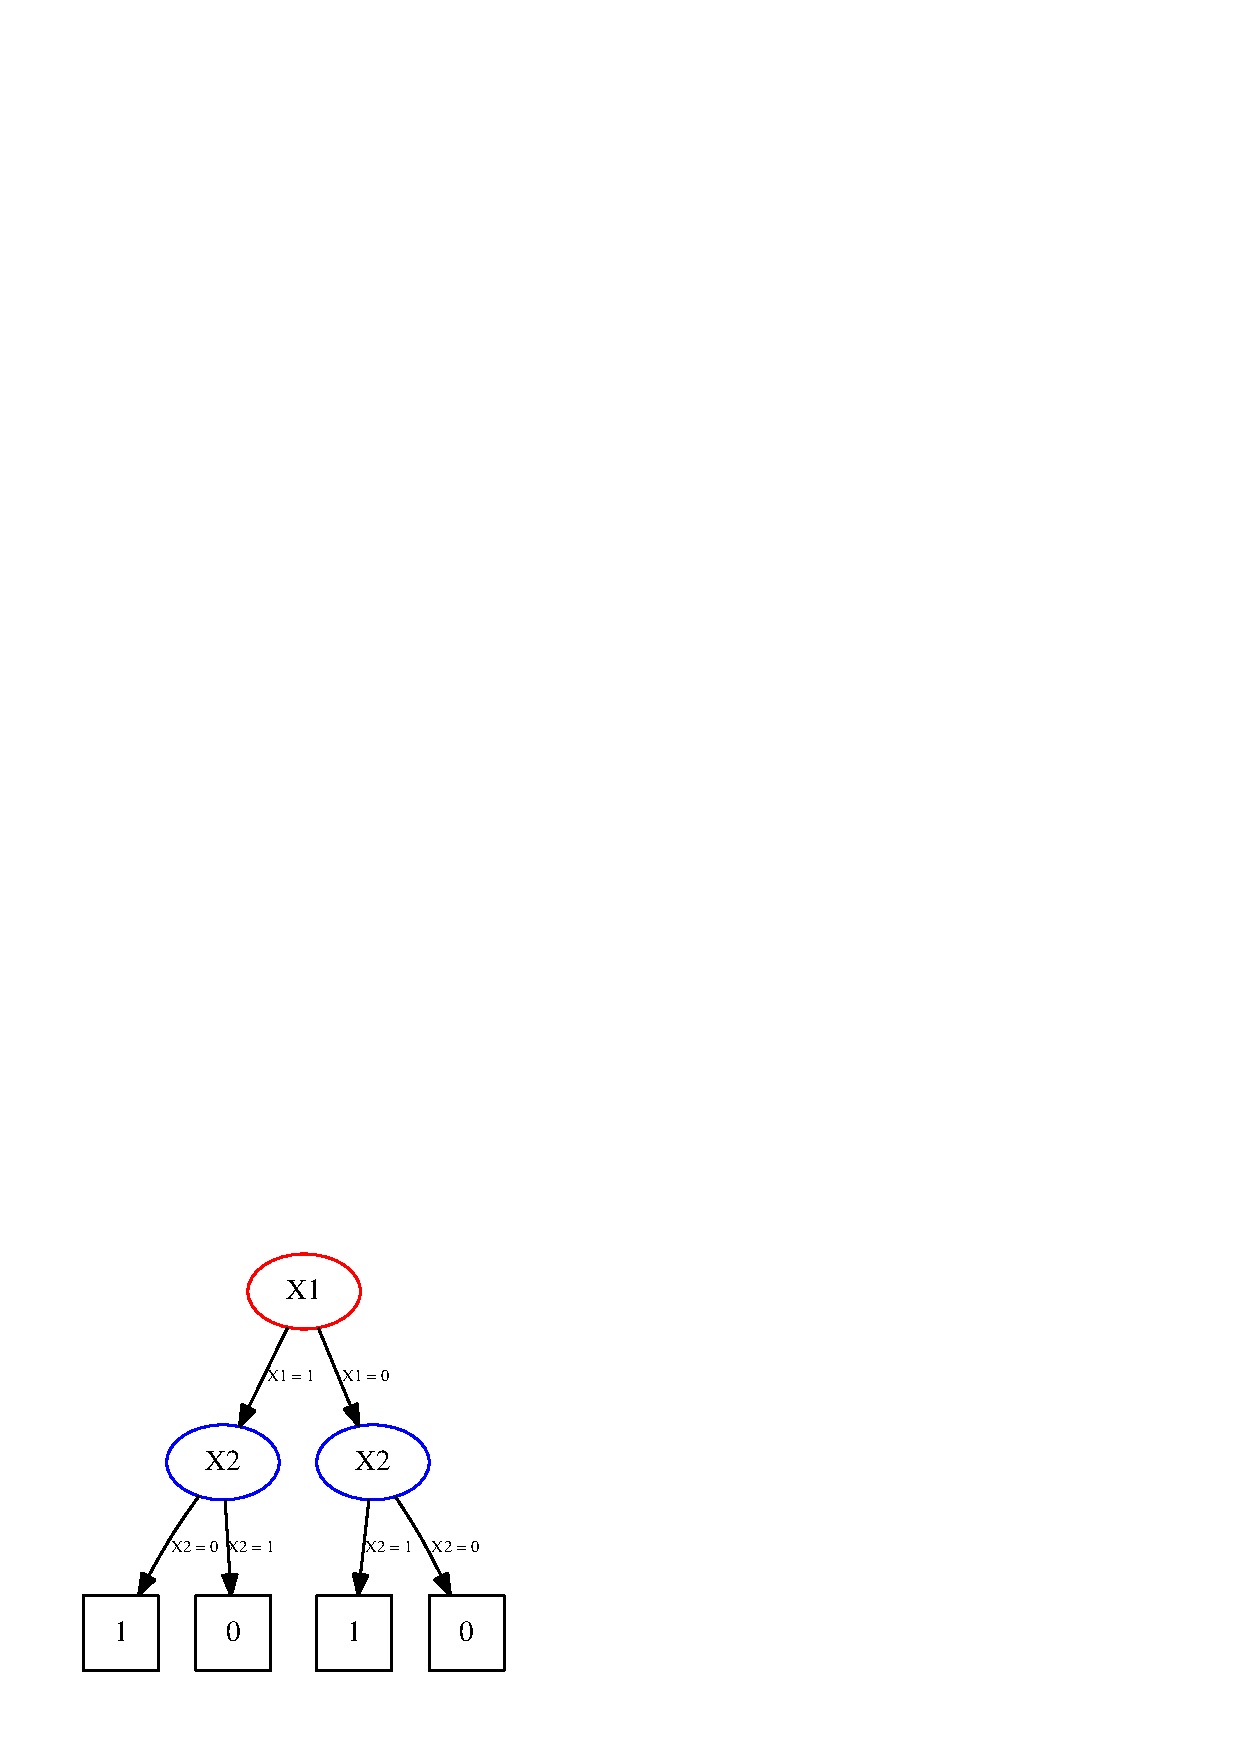
\includegraphics[width=\linewidth]{progs/1b.pdf}
  \captionof{figure}{Solution to Problem 2}
  \label{fig:1b}
\end{minipage}
\end{figure}

\begin{figure}[!h]
\centering
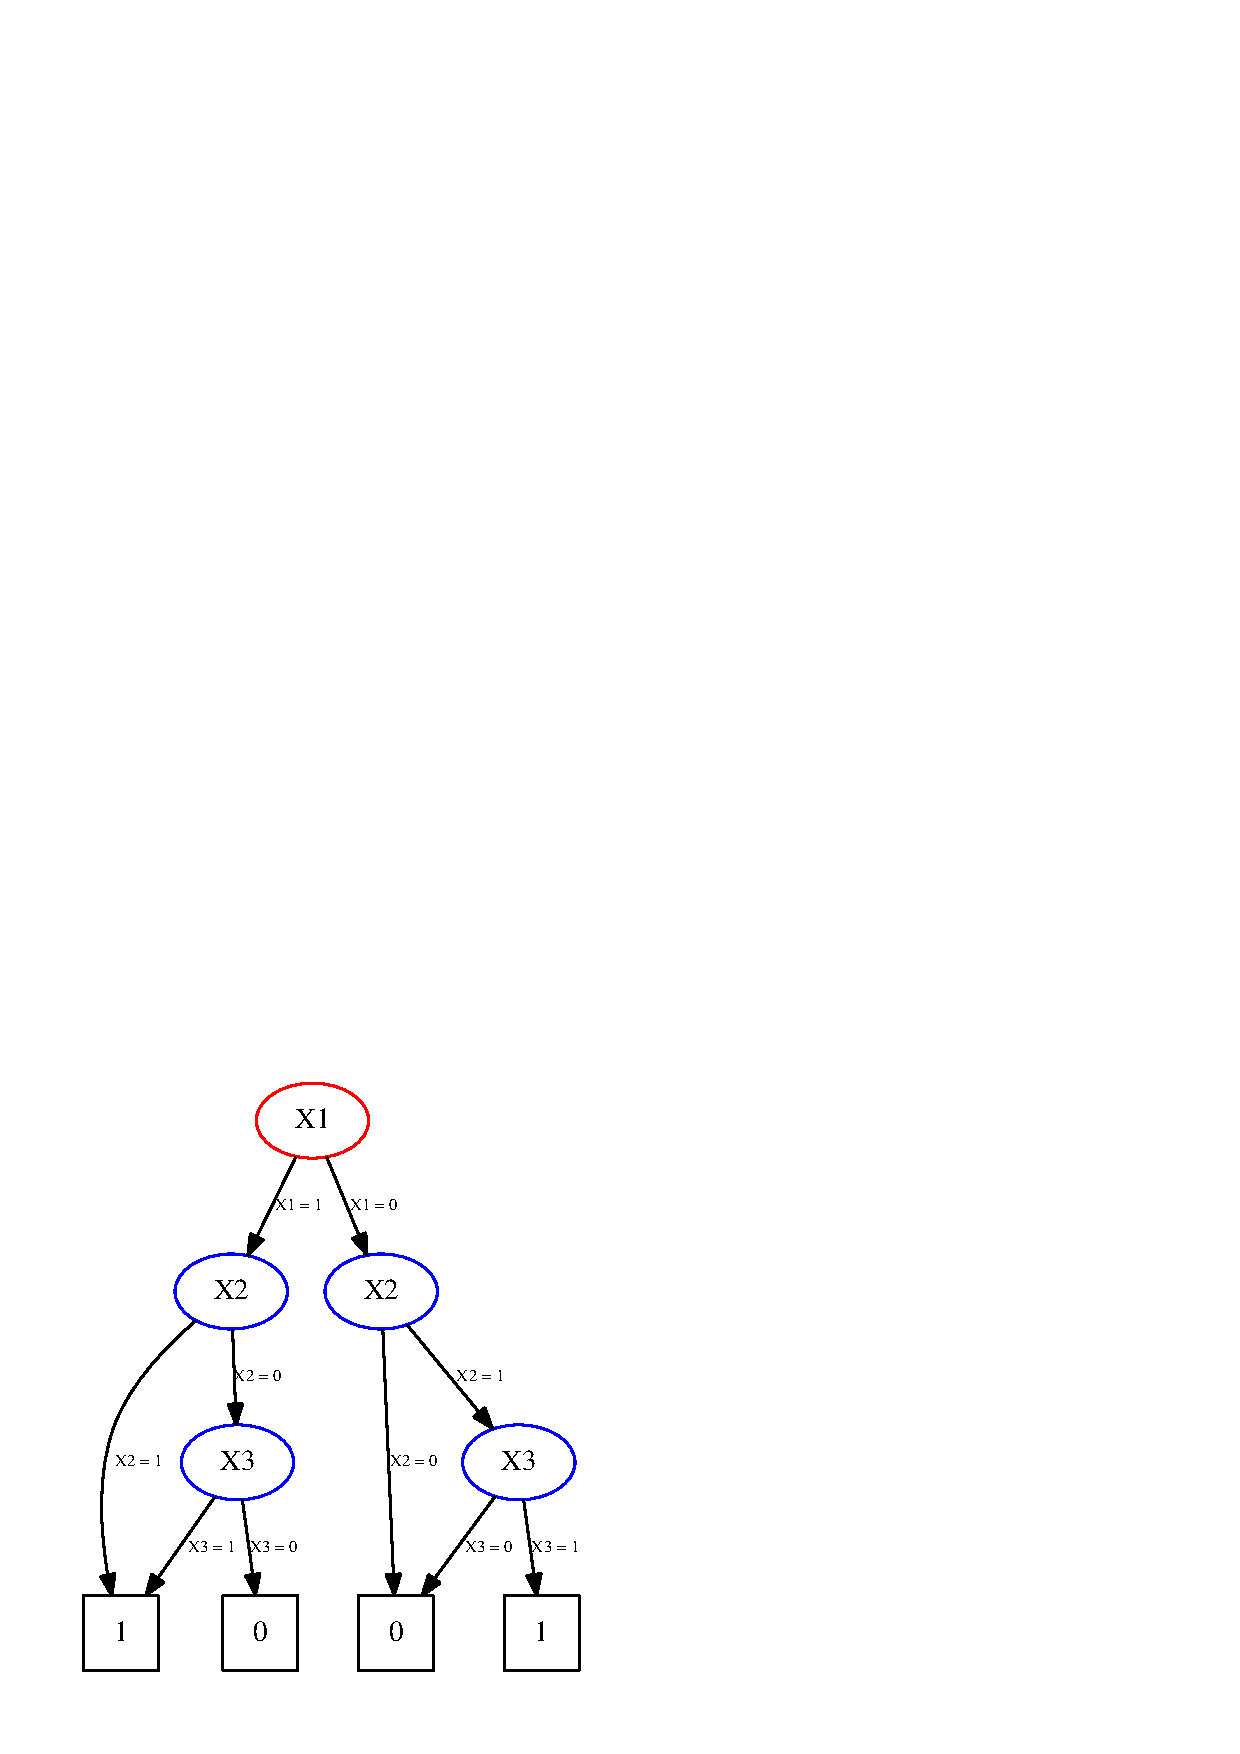
\includegraphics[width=.5\linewidth]{progs/1c.pdf}
\caption{Solution to Problem 3}
\label{fig:1c}
\end{figure}


%%% Local Variables:
%%% mode: latex
%%% TeX-master: "hw4"
%%% End:
